\documentclass{article}

% if you need to pass options to natbib, use, e.g.:
% \PassOptionsToPackage{numbers, compress}{natbib}
% before loading nips_2018

% ready for submission
\usepackage[final]{nips_2018}

% to compile a preprint version, e.g., for submission to arXiv, add
% add the [preprint] option:
% \usepackage[preprint]{nips_2018}

% to compile a camera-ready version, add the [final] option, e.g.:
% \usepackage[final]{nips_2018}

% to avoid loading the natbib package, add option nonatbib:
% \usepackage[nonatbib]{nips_2018}

\usepackage[utf8]{inputenc} % allow utf-8 input
\usepackage[T1]{fontenc}    % use 8-bit T1 fonts
\usepackage{hyperref}       % hyperlinks
\usepackage{url}            % simple URL typesetting
\usepackage{booktabs}       % professional-quality tables
\usepackage{amsfonts}       % blackboard math symbols
\usepackage{nicefrac}       % compact symbols for 1/2, etc.
\usepackage{microtype}      % microtypography
\usepackage{tabularx}
\usepackage{tikz}

\title{Increasing Entropy in a Recurrent Neural Network for Better Music Sequencing in Playlists}

% The \author macro works with any number of authors. There are two
% commands used to separate the names and addresses of multiple
% authors: \And and \AND.
%
% Using \And between authors leaves it to LaTeX to determine where to
% break the lines. Using \AND forces a line break at that point. So,
% if LaTeX puts 3 of 4 authors names on the first line, and the last
% on the second line, try using \AND instead of \And before the third
% author name.

\author{
  Trevor Jerome\\
  South Dakota School of Mines and Technology\\
  Rapid City, SD 57701 \\
  \texttt{trevor.jerome@mines.sdsmt.edu} \\
}

\begin{document}
% \nipsfinalcopy is no longer used

\maketitle

\begin{abstract}
This paper proposes a method of organizing music within playlists to emulate the organization in professionally designed albums. This is done by using a bidirectional recurrent neural network to map shuffled albums back to their original order. By doing this, it learns the structure of a good musical sequence and will recreate it on songs picked by a user in their playlist. The network begins by reading unshuffled albums and gradually moves on to more difficult problems as training goes on. This has vastly improved the performance.
\end{abstract}

\section{Introduction}
With the rise of music streaming services such as Spotify and Apple Music, people have greater access to a large variety of music than ever before. This, coupled with a plethora of music recommendation software, allows music enthusiasts to acquire vast quantities of songs in their personal collections. As with any large dataset, music libraries must be organized to achieve the greatest usefulness. It is common practice for users to organize their libraries into containers of similar songs, known as playlists. When the user then wishes to listen to their music, they will select a desired playlist to fit their mood and hit the play button on the first track.

Unfortunately, with this method, music organization begins and ends at the playlist level. Very often, the only structure \emph{within} a playlist is the order in which the user added the tracks, which most often is simply the order that the user discovered the songs. Listening to music in this order is hardly ever engaging. Songs with very different styles may be played in sequence, which can shock a listener. Conversely, songs that are too similar may become boring if played for too long. Music possesses a natural flow, and it can be unpleasant to hear if that flow is broken.

A common workaround to avoid long stretches of similar sounding songs is the "shuffle" option found in most music players. With shuffle turned on, playlists are no longer played in order, but rather songs are randomly selected from any location in the playlist. Unfortunately, this is no guarantee of avoiding the problem, and it does absolutely nothing to avoid playing dissimilar tracks back to back. In fact, it usually exacerbates this issue.

The way most music streamers help solve this problem is to provide professionally curated playlists for their users. Services such as Spotify hire producers to handpick and organize songs for maximum musical effect. Similarly, the music albums released by artists have been curated in a similar way. Given the vast number of albums present on music streaming services, it should be possible to train a neural network on these albums to recognize the characteristics of a good musical sequence and reproduce that in a playlist. Strategies for the implementation of such a network will be explored in this paper.

\section{Method}
For this problem, it is helpful to think of a raw playlist as an album that has been shuffled into a random order. The user has created their list of songs to be organized into an album, now the tracks just need to be placed in their proper sequence. To train a neural network to do this last step, then, would require feeding it albums that have been rearranged and teaching it to return them to their original order. This randomization of the input data will be done in a special way, discussed in Section \ref{sec:entropy}.

\subsection{Data Acquisition and Pre-Processing}
The data used to train this network was gathered from the Spotify API. This music streaming service provides keys to their database freely through their developer website\footnotemark. This allows developers to access an astounding amount of data on every track in Spotify's large library. This dataset was chosen over other music data, such as the Million Song Dataset, because Spotify has the capability to query albums and easily maintain the album structure. This is absolutely necessary for this project.

Using the Spotify API, data on nearly four thousand albums were retrieved. Because of the wide variety of music in existence, it was deemed appropriate to use albums most related to the tracks being organized. For this reason, the specific albums in the dataset were selected based on the artists' presence in a test playlist. Albums produced by artists suggested through Spotify's "Related Artists" feature were then chosen to increase the quantity of data. Ten percent of the albums were removed from the main training set to be included in the test set.

Each of these albums was then reduced to a matrix representation, with the first dimension representing the track at the given position and the second a vector representation of that track. These song vectors consisted of thirteen features lifted from the Spotify API. Details on these features are shown in Table \ref{tab:features}.

Because of the wide range of features included in the song vectors, normalization of the data was required. Simply calculating a global mean and standard deviation for each of the thirteen features and casting each to a unit Gaussian distribution was sufficient.

\footnotetext{https://developer.spotify.com}

\begin{table}
  \caption{Song Features \cite{2018Spotify}}
  \label{tab:features}
  \centering
  \begin{tabularx}{\linewidth}{lX}
    \toprule
    Name     & Description \\
    \midrule
    Acousticness & A measure from 0.0 to 1.0 of the confidence of the track being acoustic. \\
    Danceability & A measure from 0.0 to 1.0 of how suitable the track is for dancing. Based on a combination of many musical elements. \\
    Duration & The length of the track in milliseconds. \\
    Energy & A measure from 0.0 to 1.0 of the intensity of the track. Based on a combination of many musical elements. \\
    Instrumentalness & A measure from 0.0 to 1.0 of the confidence of the track containing no vocals. \\
    Key & An integer value representing the musical key of the track, following standard Pitch Class Notation. \\
    Liveness & A measure from 0.0 to 1.0 of the confidence of the track containing an audience. \\
    Loudness & The average volume of the track in decibels. \\
    Mode & An integer representing the modality of the track. Major is represented by a 1, and minor by a 0. \\
    Speechiness & A measure from 0.0 to 1.0 of the presence of spoken word in the track. \\
    Tempo & The tempo of the track in beats per minute. \\
    Time Signature & The number of beats in each musical measure. \\
    Valence & A measure from 0.0 to 1.0 of the positivity of the track. \\
    \bottomrule
  \end{tabularx}
\end{table}

\subsection{Network}
Because the problem requires processing sequences of data, a recurrent neural network (RNN) is the best fit for the job. Because albums can be of many varying lengths, a dynamically sized network is needed. In order to avoid long sequences of similar sounding songs, the network needs to be able to remember earlier in the sequence. This means that an LSTM cell is perfect for the job \cite{Olah2015Understanding}.

This network was implemented using Tensorflow's bidirectional dynamic RNN with a hidden size of one thousand. A 50\% dropout was added as regularization. The dropout mask remained the same over every time step of the RNN to increase performance, as suggested by Gal and Ghahramani \cite{Gal2016Theoretically}.

The RNN outputs a matrix with a value between 0.0 and 1.0 for each track and location in the album. This value represents the confidence of a given track belonging in a specific position. Finally, the Adam optimization algorithm with a cross-entropy loss function was used to refine the network. Adam was chosen due to its specialization in dealing with low gradients and noisy data \cite{2017Adam}. Other algorithms were tested alongside Adam and did not compare in performance.

\subsection{Increasing Entropy}
\label{sec:entropy}
Before the input data is fed into the network, it needs to be shuffled up. However, in testing the network struggled to apply what it learned on the test dataset. This was likely because it simply memorized the intended sequence for every given album. To counteract this, the data was reshuffled before every training epoch so that the network was forced to learn proper sequencing rather than just memorization. Unfortunately, with this method the network could not learn anything at all and resorted to guessing the same song for every position in the album.

The problem was solved by writing a function to take a parameter called "entropy" and shuffle the albums to a varying degree based on this parameter. Entropy is a float value from 0.0 to 1.0 that corresponds to the degree of shuffling within each album. It is multiplied by the length of the album to determine the number of swaps to be performed on album indices. An index vector is generated with $n$ random integers, where $n = 2 \times swaps$ and the random numbers fall in the range of album indices to be shuffled. These indices are then popped off two at time, and the two corresponding tracks in the album are swapped. Entropy values below 0.5 only perform one sequence of swaps. From 0.5 to 1.0, two sequences of swaps are done. Figure \ref{fig:shuffling} demonstrates this method. Note that for this application, the first and last values are left untouched, because the user will be able to select the start and end points of their playlist. This restriction does not have to exist in other applications.

This entropy value is then increased throughout training, saturating at a certain point and shuffling the albums completely from that point onward. This allowed the network time to learn the sequence data before gradually easing into the unshuffling operations. The saturation point is chosen as a hyperparameter. Generally, earlier saturation points work better, allowing the network to spend more time learning sequences of fully shuffled data.

\begin{figure}

\tikzset{every picture/.style={line width=0.75pt}} %set default line width to 0.75pt        
\centering
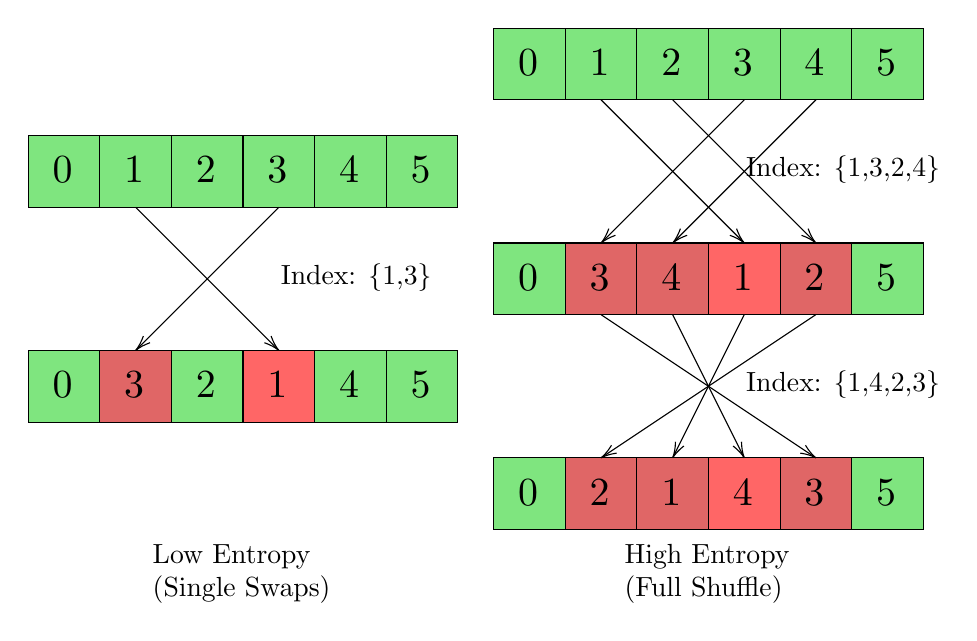
\begin{tikzpicture}[x=0.75pt,y=0.75pt,yscale=-1,xscale=1,scale=\textwidth/500]
\draw    (401,51) -- (501,151) ;
\draw [shift={(501,151)}, rotate = 225] [color={rgb, 255:red, 0; green, 0; blue, 0 }  ]   (0,0) .. controls (3.31,-0.3) and (6.95,-1.4) .. (10.93,-3.29)(0,0) .. controls (3.31,0.3) and (6.95,1.4) .. (10.93,3.29)   ;

\draw    (501,51) -- (401,151) ;
\draw [shift={(401,151)}, rotate = 315] [color={rgb, 255:red, 0; green, 0; blue, 0 }  ]   (0,0) .. controls (3.31,-0.3) and (6.95,-1.4) .. (10.93,-3.29)(0,0) .. controls (3.31,0.3) and (6.95,1.4) .. (10.93,3.29)   ;

\draw    (551,51) -- (451,151) ;
\draw [shift={(451,151)}, rotate = 315] [color={rgb, 255:red, 0; green, 0; blue, 0 }  ]   (0,0) .. controls (3.31,-0.3) and (6.95,-1.4) .. (10.93,-3.29)(0,0) .. controls (3.31,0.3) and (6.95,1.4) .. (10.93,3.29)   ;

\draw    (451,51) -- (551,151) ;
\draw [shift={(551,151)}, rotate = 225] [color={rgb, 255:red, 0; green, 0; blue, 0 }  ]   (0,0) .. controls (3.31,-0.3) and (6.95,-1.4) .. (10.93,-3.29)(0,0) .. controls (3.31,0.3) and (6.95,1.4) .. (10.93,3.29)   ;

\draw    (501,201) -- (451,301) ;
\draw [shift={(451,301)}, rotate = 296.57] [color={rgb, 255:red, 0; green, 0; blue, 0 }  ]   (0,0) .. controls (3.31,-0.3) and (6.95,-1.4) .. (10.93,-3.29)(0,0) .. controls (3.31,0.3) and (6.95,1.4) .. (10.93,3.29)   ;

\draw    (551,201) -- (401,301) ;
\draw [shift={(401,301)}, rotate = 326.31] [color={rgb, 255:red, 0; green, 0; blue, 0 }  ]   (0,0) .. controls (3.31,-0.3) and (6.95,-1.4) .. (10.93,-3.29)(0,0) .. controls (3.31,0.3) and (6.95,1.4) .. (10.93,3.29)   ;

\draw    (451,201) -- (501,301) ;
\draw [shift={(501,301)}, rotate = 243.43] [color={rgb, 255:red, 0; green, 0; blue, 0 }  ]   (0,0) .. controls (3.31,-0.3) and (6.95,-1.4) .. (10.93,-3.29)(0,0) .. controls (3.31,0.3) and (6.95,1.4) .. (10.93,3.29)   ;

\draw    (401,201) -- (551,301) ;
\draw [shift={(551,301)}, rotate = 213.69] [color={rgb, 255:red, 0; green, 0; blue, 0 }  ]   (0,0) .. controls (3.31,-0.3) and (6.95,-1.4) .. (10.93,-3.29)(0,0) .. controls (3.31,0.3) and (6.95,1.4) .. (10.93,3.29)   ;

\draw    (76,126) -- (176,226) ;
\draw [shift={(176,226)}, rotate = 225] [color={rgb, 255:red, 0; green, 0; blue, 0 }  ]   (0,0) .. controls (3.31,-0.3) and (6.95,-1.4) .. (10.93,-3.29)(0,0) .. controls (3.31,0.3) and (6.95,1.4) .. (10.93,3.29)   ;

\draw    (176,126) -- (76,226) ;
\draw [shift={(76,226)}, rotate = 315] [color={rgb, 255:red, 0; green, 0; blue, 0 }  ]   (0,0) .. controls (3.31,-0.3) and (6.95,-1.4) .. (10.93,-3.29)(0,0) .. controls (3.31,0.3) and (6.95,1.4) .. (10.93,3.29)   ;

\draw  [fill={rgb, 255:red, 0; green, 204; blue, 0 }  ,fill opacity=0.5 ]  (1, 226) rectangle (51, 276)   ;
\draw  [fill={rgb, 255:red, 204; green, 0; blue, 0 }  ,fill opacity=0.6 ]  (51, 226) rectangle (101, 276)   ;
\draw  [fill={rgb, 255:red, 0; green, 204; blue, 0 }  ,fill opacity=0.5 ]  (101, 226) rectangle (151, 276)   ;
\draw  [fill={rgb, 255:red, 255; green, 0; blue, 0 }  ,fill opacity=0.6 ]  (151, 226) rectangle (201, 276)   ;
\draw  [fill={rgb, 255:red, 0; green, 204; blue, 0 }  ,fill opacity=0.5 ]  (201, 226) rectangle (251, 276)   ;
\draw  [fill={rgb, 255:red, 0; green, 204; blue, 0 }  ,fill opacity=0.5 ]  (251, 226) rectangle (301, 276)   ;
\draw  [fill={rgb, 255:red, 0; green, 204; blue, 0 }  ,fill opacity=0.5 ]  (1, 76) rectangle (51, 126)   ;
\draw  [fill={rgb, 255:red, 0; green, 204; blue, 0 }  ,fill opacity=0.5 ]  (51, 76) rectangle (101, 126)   ;
\draw  [fill={rgb, 255:red, 0; green, 204; blue, 0 }  ,fill opacity=0.5 ]  (101, 76) rectangle (151, 126)   ;
\draw  [fill={rgb, 255:red, 0; green, 204; blue, 0 }  ,fill opacity=0.5 ]  (151, 76) rectangle (201, 126)   ;
\draw  [fill={rgb, 255:red, 0; green, 204; blue, 0 }  ,fill opacity=0.5 ]  (201, 76) rectangle (251, 126)   ;
\draw  [fill={rgb, 255:red, 0; green, 204; blue, 0 }  ,fill opacity=0.5 ]  (251, 76) rectangle (301, 126)   ;

\draw  [fill={rgb, 255:red, 0; green, 204; blue, 0 }  ,fill opacity=0.5 ]  (326, 151) rectangle (376, 201)   ;
\draw  [fill={rgb, 255:red, 204; green, 0; blue, 0 }  ,fill opacity=0.6 ]  (376, 151) rectangle (426, 201)   ;
\draw  [fill={rgb, 255:red, 204; green, 0; blue, 0 }  ,fill opacity=0.6 ]  (426, 151) rectangle (476, 201)   ;
\draw  [fill={rgb, 255:red, 255; green, 0; blue, 0 }  ,fill opacity=0.6 ]  (476, 151) rectangle (526, 201)   ;
\draw  [fill={rgb, 255:red, 204; green, 0; blue, 0 }  ,fill opacity=0.6 ]  (526, 151) rectangle (576, 201)   ;
\draw  [fill={rgb, 255:red, 0; green, 204; blue, 0 }  ,fill opacity=0.5 ]  (576, 151) rectangle (626, 201)   ;
\draw  [fill={rgb, 255:red, 0; green, 204; blue, 0 }  ,fill opacity=0.5 ]  (326, 1) rectangle (376, 51)   ;
\draw  [fill={rgb, 255:red, 0; green, 204; blue, 0 }  ,fill opacity=0.5 ]  (376, 1) rectangle (426, 51)   ;
\draw  [fill={rgb, 255:red, 0; green, 204; blue, 0 }  ,fill opacity=0.5 ]  (426, 1) rectangle (476, 51)   ;
\draw  [fill={rgb, 255:red, 0; green, 204; blue, 0 }  ,fill opacity=0.5 ]  (476, 1) rectangle (526, 51)   ;
\draw  [fill={rgb, 255:red, 0; green, 204; blue, 0 }  ,fill opacity=0.5 ]  (526, 1) rectangle (576, 51)   ;
\draw  [fill={rgb, 255:red, 0; green, 204; blue, 0 }  ,fill opacity=0.5 ]  (576, 1) rectangle (626, 51)   ;
\draw  [fill={rgb, 255:red, 0; green, 204; blue, 0 }  ,fill opacity=0.5 ]  (326, 301) rectangle (376, 351)   ;
\draw  [fill={rgb, 255:red, 204; green, 0; blue, 0 }  ,fill opacity=0.6 ]  (376, 301) rectangle (426, 351)   ;
\draw  [fill={rgb, 255:red, 204; green, 0; blue, 0 }  ,fill opacity=0.6 ]  (426, 301) rectangle (476, 351)   ;
\draw  [fill={rgb, 255:red, 255; green, 0; blue, 0 }  ,fill opacity=0.6 ]  (476, 301) rectangle (526, 351)   ;
\draw  [fill={rgb, 255:red, 204; green, 0; blue, 0 }  ,fill opacity=0.6 ]  (526, 301) rectangle (576, 351)   ;
\draw  [fill={rgb, 255:red, 0; green, 204; blue, 0 }  ,fill opacity=0.5 ]  (576, 301) rectangle (626, 351)   ;

\draw (25,100) node [scale=1.44] [align=left] {0};
\draw (75,100) node [scale=1.44] [align=left] {1};
\draw (125,100) node [scale=1.44] [align=left] {2};
\draw (175,100) node [scale=1.44] [align=left] {3};
\draw (225,100) node [scale=1.44] [align=left] {4};
\draw (275,100) node [scale=1.44] [align=left] {5};
\draw (150,382) node  [align=left] {Low Entropy\\(Single Swaps)};
\draw (475,382) node  [align=left] {High Entropy\\(Full Shuffle)};
\draw (350,175) node [scale=1.44] [align=left] {0};
\draw (400,175) node [scale=1.44] [align=left] {3};
\draw (450,175) node [scale=1.44] [align=left] {4};
\draw (500,175) node [scale=1.44] [align=left] {1};
\draw (550,175) node [scale=1.44] [align=left] {2};
\draw (600,175) node [scale=1.44] [align=left] {5};
\draw (350,25) node [scale=1.44] [align=left] {0};
\draw (400,25) node [scale=1.44] [align=left] {1};
\draw (450,25) node [scale=1.44] [align=left] {2};
\draw (500,25) node [scale=1.44] [align=left] {3};
\draw (550,25) node [scale=1.44] [align=left] {4};
\draw (600,25) node [scale=1.44] [align=left] {5};
\draw (350,325) node [scale=1.44] [align=left] {0};
\draw (400,325) node [scale=1.44] [align=left] {2};
\draw (450,325) node [scale=1.44] [align=left] {1};
\draw (500,325) node [scale=1.44] [align=left] {4};
\draw (550,325) node [scale=1.44] [align=left] {3};
\draw (600,325) node [scale=1.44] [align=left] {5};
\draw (25,250) node [scale=1.44] [align=left] {0};
\draw (75,250) node [scale=1.44] [align=left] {3};
\draw (125,250) node [scale=1.44] [align=left] {2};
\draw (175,250) node [scale=1.44] [align=left] {1};
\draw (225,250) node [scale=1.44] [align=left] {4};
\draw (275,250) node [scale=1.44] [align=left] {5};
\draw (230,175) node  [align=left] {Index: \{1,3\}};
\draw (570,250) node  [align=left] {Index: \{1,4,2,3\}};
\draw (570,100) node  [align=left] {Index: \{1,3,2,4\}};

\end{tikzpicture}

\caption{Entropy-based Shuffling Method}
\label{fig:shuffling}

\end{figure}

\section{Experiments and Results}

\subsection{Data Pre-Processing}
Data normalization proved to be very important for this project. This is not surprising, given the wide range of values included in the song vectors. Figure \ref{fig:nonorm} shows the error in both the test set and the training set, sampled every 100 epochs. This error is measured as the percentage of songs in the entire dataset that were placed in their correct position in their album. The error in this particular training session shows that, even after 5,000 epochs of training, the network has still not managed to make the weights fit the data, meaning that normalization is desperately needed. The rest of the error graphs in this section show the network's performance on normalized data, which is significantly better.

\begin{figure}
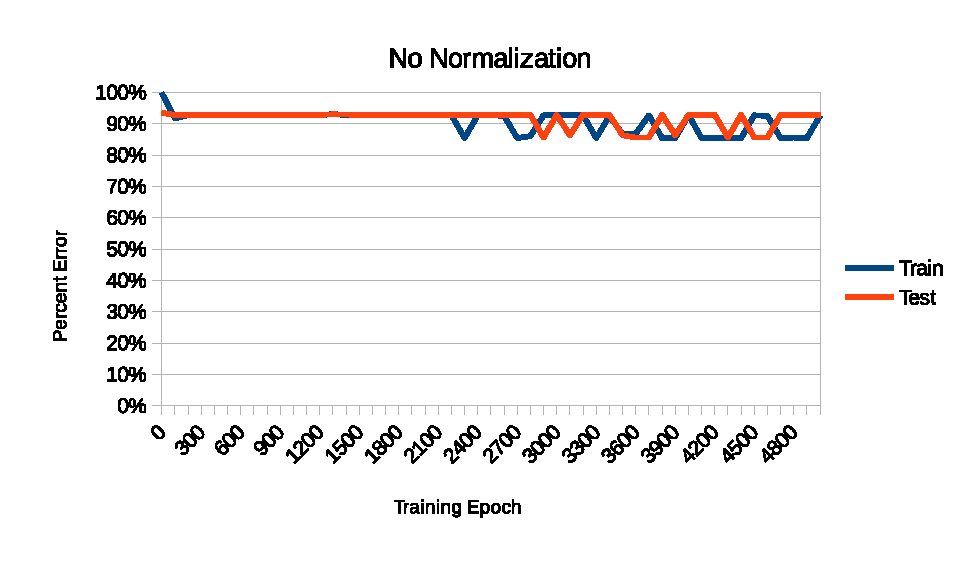
\includegraphics[width=\textwidth]{No-Normalization.eps}
\caption{Error graph with no normalization}
\label{fig:nonorm}
\end{figure}
\subsection{Optimizers}
Before the Adam optimizer was chosen, both Gradient Descent and Adagrad were tested on the network. Their results, only shuffling the data once at pre-processing, are shown if Figure \ref{fig:optimizers}. Results using Adam are shown in Figures \ref{fig:normalreg} and \ref{fig:entropy}. Clearly, Adam is the best fit for this application.

\begin{figure}
%\centering
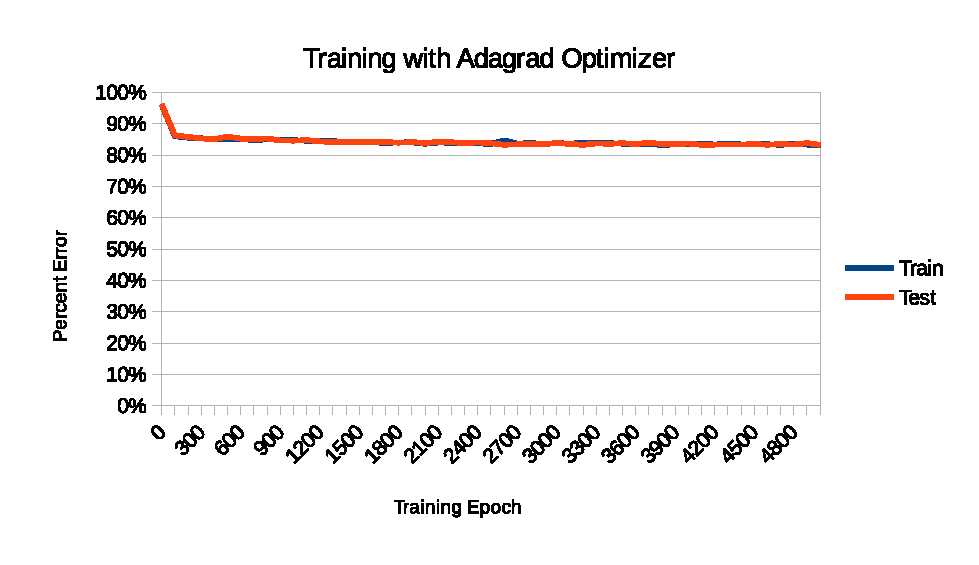
\includegraphics[width=.5\textwidth]{Adagrad.eps}
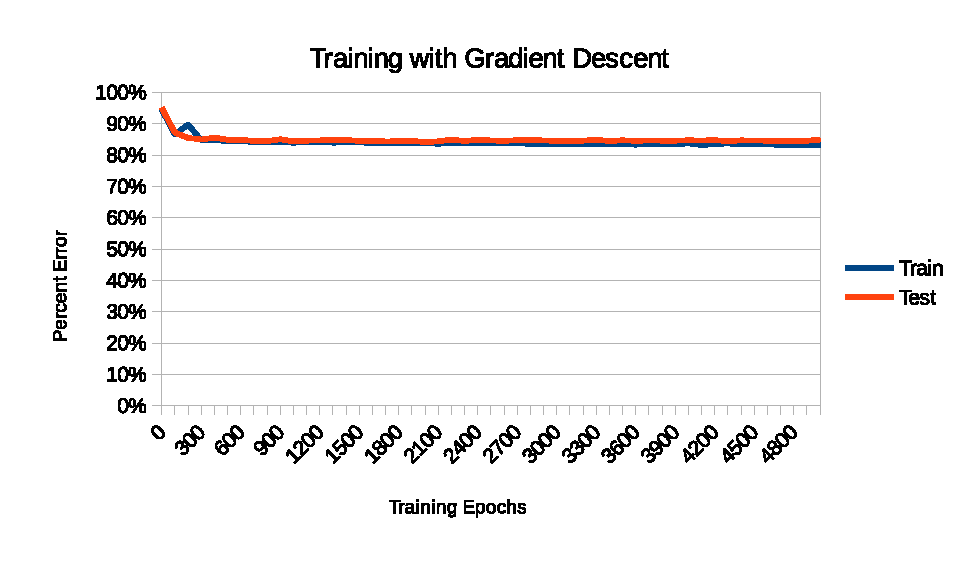
\includegraphics[width=.5\textwidth]{Gradient-Descent.eps}
\caption{Error graphs from other optimization algorithms: (top) Adagrad, and (bottom) gradient descent.}
\label{fig:optimizers}
\end{figure}
\subsection{Increasing Entropy}
As stated in Section \ref{sec:entropy}, the network was experiencing a great deal of trouble learning to unshuffle albums with standard methods of regularization. Figure \ref{fig:normalreg} shows the error graph for one of each of these tests. Neither method yielded any reduction of error in the test set beyond the first few epochs. When shuffling at each batch, the network could not even learn on the training set.

With the method of increasing entropy, the network was able to briefly look at the albums' intended structure before being forced to learn more complicated aspects of the musical flow. Figure \ref{fig:entropy} shows the results of this. It should be noted that all error estimates were done on fully shuffled data. It is interesting to see the uptick in the training error as the network figures out that a straight sequence will no longer work. When the training error begins to decrease the second time, the test error begins to decrease much faster. This shows that the network is now working as intended.

Unfortunately, there was not enough time available to perform full length tests on this network to see if it could reduce the error much further. The longest test performed was 250,000 epochs with an entropy saturation point of 12,000 epochs. This yielded a 57.6\% error on the test set. It was performed on an NVIDIA 1060 GeForce with 6GB of memory and took twelve hours to complete. Similar models using a bidirectional recurrent neural network have taken eight weeks to complete training \cite{NIPS2015_5651}. Given that the error in Figure \ref{fig:entropy} is still decreasing at the end of its training, it is likely that a longer test will yield much better results.

\begin{figure}
%\centering
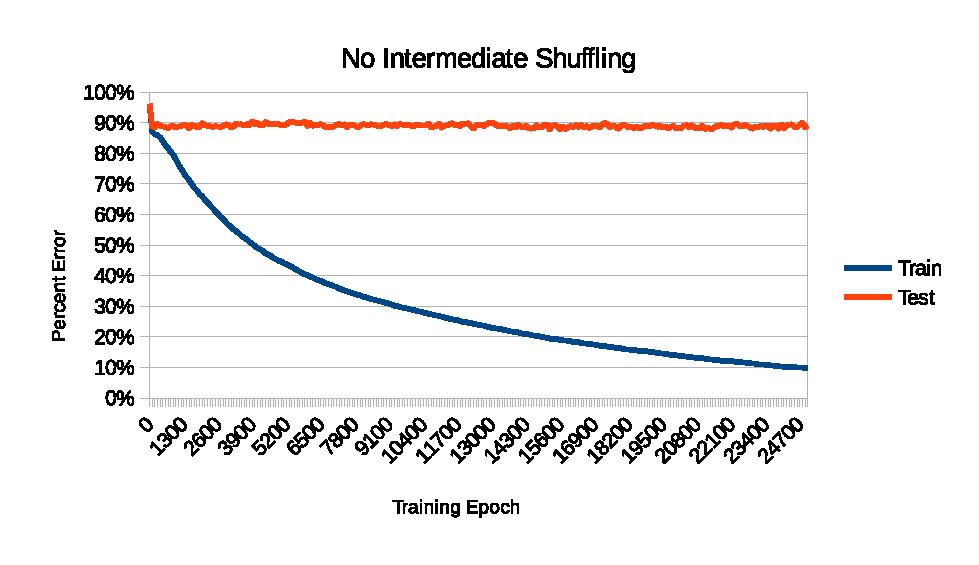
\includegraphics[width=.5\textwidth]{No-Intermediate-Shuffling.eps}
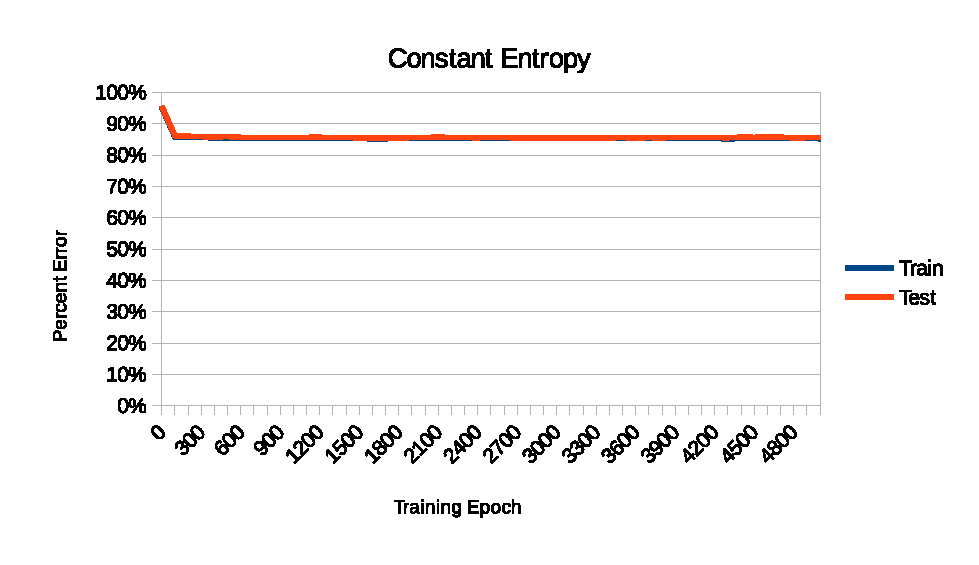
\includegraphics[width=.5\textwidth]{Constant-Entropy.eps}
\caption{Error graphs from normal shuffling methods: (top) shuffling once at the pre-processing stage, and (bottom) shuffling at each batch.}
\label{fig:normalreg}
\end{figure}
\begin{figure}
\centering
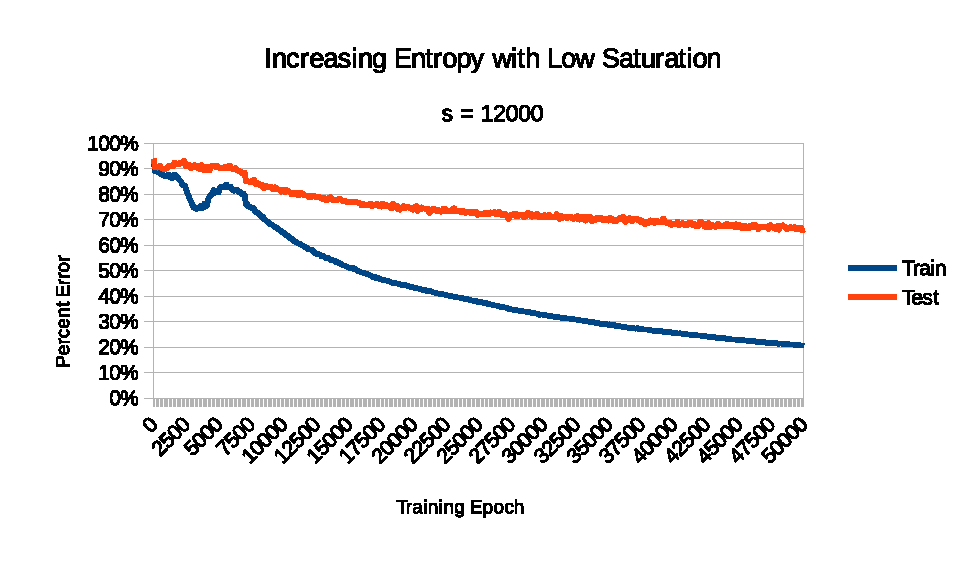
\includegraphics[width=.75\textwidth]{Increasing-Entropy.eps}
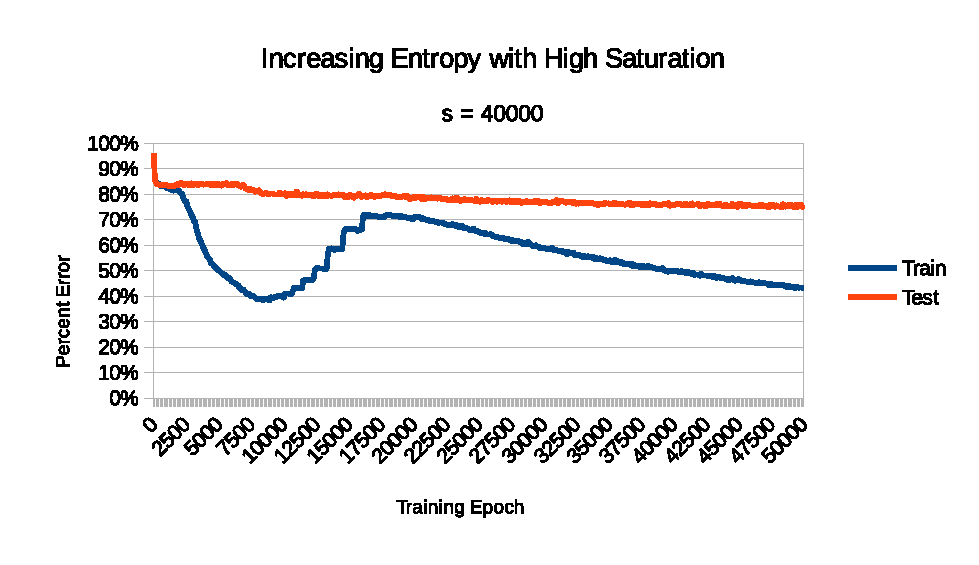
\includegraphics[width=.75\textwidth]{High-Saturation.eps}
\caption{Error graphs from increasing entropy with each epoch, showing results with a (top) low saturation point, and (bottom) high saturation point.}
\label{fig:entropy}
\end{figure}

\section{Future Work}
Obviously, there is a lot of work still to be done on this problem. The current level of error renders it unusable for the intended application. However, it shows promise given more time to implement improvements.

\paragraph{Restrict Duplicates} In music albums, tracks are never repeated. However, there is currently no restriction on duplicates within this network. Implementing this would likely lead to lower error, since looking at the predictions shows that many tracks are predicted to be in multiple locations within the album. One way this could be done is by modifying the loss function to include a count of duplicate items within each prediction. This would allow the RNN to minimize the number of duplicates by itself. Another method would be to add a regression layer after the RNN to select the linear sequence that minimizes the mean squared error between each selected value and its confidence level in the prediction matrix.

\paragraph{Refine Hyperparameters} Because of the limited time to test the network and long training times, it was difficult to find the optimal combination of hyperparameters. Some data was gathered that could lead to better training in the future. For instance, a large number of nodes in the RNN seems to train faster. The training rate cannot get to be much more than 0.001 without diverging. Finally, as shown earlier, a low entropy saturation point gives the best results. More thorough testing of these hyperparameters will give better performance of the network in the future.

\paragraph{Longer Testing} Finally, a testing period of many days may be all that is needed to bring the error to acceptable levels. Because this network was built in a very busy time of the year, GPU time was only available in relatively short increments. During the summer, a longer test will be possible.

\section{Conclusion}
In this paper, a bidirectional recurrent neural network was proposed to better organize playlists by attempting to recreate the structure of professionally designed albums. This will be done by training it to reverse the shuffling done on albums to learn the proper sequences by linking together sequences of song vectors. These song vectors are based on data pulled from the Spotify Web API.

Despite some earlier bumps in the road, this network is showing promise after implementing the method of increasing entropy. By allowing the network to see both the original sequences and shuffled sequences, it is able to begin to learn the flow of the album. In addition to this technique, data normalization, variational dropout, and the Adam optimizer were used to create this network. After a few more improvements and given more time to train, it will likely be a useful tool for playlist organization.

\bibliography{sources.bib}
\bibliographystyle{plain}

\end{document}
